\question[4]
Führe den Algorithmus von Bellman-Ford mit Startknoten a aus.
Notiere nach jedem Durchgang die Kosten an den Knoten

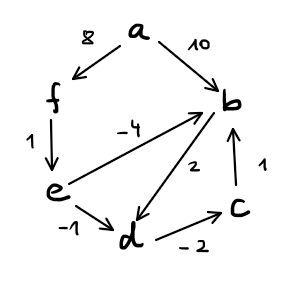
\includegraphics[height=5cm]{\pfad/Graphen/Aufgaben/bellman_03/bellman_03.png}
\begin{solutionbox}{5cm}
\begin{lstlisting}
     a  b   c   d   e   f
0 :  0  inf inf inf inf inf
1 :  0  10  10  12  9   8
2 :  0  5   10  8   9   8
3 :  0  5   5   7   9   8
4 :  0  5   5   7   9   8
\end{lstlisting}
\end{solutionbox}
